\section{Experiments}
\label{sec:experiments}
\paragraph{Tasks.}
All four tasks have a program verifier, so rewards are exact and no reward model is involved (details in Appendix~\ref{app:datasets}). \textbf{Countdown} \citep{gandhi2024sos}: reach a target from four to five numbers with $+,-,\times,\div$; the answer is a derivation. \textbf{Sudoku} \citep{shah2024sudoku}: fill a $9\times9$ grid; solutions are unique; the model emits all 81 cells. \textbf{Knights-and-Knaves} (K\&K) \citep{xie2024kk}: assign knight/knave to $n\in\{4,5,6\}$ characters from their statements; solutions are unique. \textbf{Game24} \citep{yao2023tot}: reach 24 from four numbers. Game24 has only 1{,}345 solvable number sets, so we split by \emph{set}: the 1{,}601 evaluation prompts are orderings of 269 sets the model has never seen, and more supervised fine-tuning \emph{hurts} on this split (Appendix~\ref{app:g24_sft}).

\paragraph{Models and protocol.}
Every run starts from ELF-B (105M) fine-tuned on the task with the ELF recipe, at a checkpoint with headroom (Appendix~\ref{app:details}); accuracy is measured on 2{,}000 held-out prompts (1{,}601 for Game24) under four samplers (Appendix~\ref{app:results}), of which Table~\ref{tab:main} shows the deployment sampler ($\gamma56$@64; $\gamma28$@32 on Sudoku) and Table~\ref{tab:ode} the cheap 64-step ODE sampler. GRPO is the score-function baseline in its standard form (group size 8, uniform credit over steps and positions, no KL, 600 iterations, $\gamma4$@16 rollouts, checkpoints every 100). The two \jpc{} rows follow Algorithm~\ref{alg:jpc} exactly and differ only in the critic head: the scalar critic pools the features and then applies the head, the 2D critic applies the head at every position and pools the values; pre-training rollouts, stored steps, joint training, learning-rate schedule and evaluation are identical (1000--1500 iterations, a checkpoint every 250). Every ELF-B RL row is the mean over three seeds of the per-seed peak over all saved checkpoints, every seed counted (evaluation jitter $\approx\pm0.3$); the budgets differ by estimator (GRPO $\approx$77k rollouts of 16 steps per run, \jpc{} 32--48k rollouts of 64 steps plus the critic; comparable GPU-hours, Appendix~\ref{app:details}). GPT-2 (124M) and LLaDA-8B-Instruct are trained on the same data, with token-level GRPO/PPO and with d1's diffu-GRPO (Appendices~\ref{app:ar_curves} and~\ref{app:d1}). Every loop row starts from one policy and runs the same number of rounds per task (Countdown 4, Sudoku 1, K\&K 5, Game24 4); each round fine-tunes the previous round's final checkpoint on verifier-accepted samples of a fixed problem pool, and the tables report the last round (Appendix~\ref{app:details}).

\begin{table}[t]
\centering\small
\begin{minipage}[t]{0.585\linewidth}
\centering
\caption{Held-out accuracy (\%) at the deployment sampler.}
\label{tab:main}
\resizebox{\linewidth}{!}{%
\begin{tabular}{@{}lcccc@{}}
\toprule
 & Countdown & Sudoku & K\&K & Game24 \\
\midrule
\multicolumn{5}{@{}l}{\emph{GPT-2 (124M, autoregressive)}}\\
task SFT & 44.2 & \phantom{0}1.2 & 92.9 & 26.9 \\
+ token-level GRPO/PPO & 53.9 & \phantom{0}1.4 & 93.2 & 32.2 \\
\midrule
\multicolumn{5}{@{}l}{\emph{LLaDA-8B-Instruct (masked diffusion)}}\\
task SFT & 13.1 & \phantom{0}0.7 & 61.0 & 16.1 \\
+ diffu-GRPO & \PENDcd & \phantom{0}0.7 & 62.5 & 19.5 \\
\midrule
\multicolumn{5}{@{}l}{\emph{ELF-B (105M, continuous flow)}}\\
task SFT (base) & 42.2 & 66.2 & 67.5 & 45.0 \\
+ GRPO & 43.1 & 69.7 & 71.6 & 47.5 \\
+ \jpc{}, scalar critic & \textbf{48.5} & 67.4 & 78.2 & 51.9 \\
+ \hl{\jpc{}, 2D critic} & 46.9 & \textbf{70.0} & \textbf{79.2} & \textbf{58.9} \\
\midrule
\multicolumn{5}{@{}l}{\emph{ELF-B, amortisation loop (4 / 1 / 5 / 4 rounds)}}\\
loop from the SFT base (no RL) & \LOOPcdB & 65.5 & \LOOPkkB & 46.1 \\
loop from the GRPO policy & 45.1 & \textbf{71.9} & \LOOPkkG & 50.5 \\
gold labels of the loop's problems (oracle) & 43.1 & 70.5 & \textbf{99.8} & 49.5 \\
\hl{2D-critic policy + loop} & \textbf{52.3} & 70.8 & 98.8 & \textbf{58.1} \\
\bottomrule
\end{tabular}}
\end{minipage}\hfill
\begin{minipage}[t]{0.40\linewidth}
\centering
\caption{ELF-B at the cheap 64-step ODE sampler (\%).}
\label{tab:ode}
\resizebox{\linewidth}{!}{%
\begin{tabular}{@{}lcccc@{}}
\toprule
 & Countdown & Sudoku & K\&K & Game24 \\
\midrule
task SFT (base) & 28.1 & 62.3 & 57.8 & 35.2 \\
+ GRPO & 28.9 & \textbf{66.0} & 63.7 & 36.5 \\
+ \jpc{}, scalar critic & \textbf{33.5} & 64.3 & \textbf{69.1} & 38.6 \\
+ \hl{\jpc{}, 2D critic} & 33.3 & 65.2 & \textbf{69.1} & \textbf{41.2} \\
\midrule
loop from the SFT base & \LOOPcdBo & 62.0 & \LOOPkkBo & 40.2 \\
loop from the GRPO policy & 42.1 & \textbf{68.5} & \LOOPkkGo & 43.5 \\
gold labels (oracle) & 27.5 & 66.5 & \textbf{97.7} & 39.4 \\
\hl{2D-critic policy + loop} & \textbf{49.5} & 66.1 & 95.2 & \textbf{50.9} \\
\bottomrule
\end{tabular}}
\end{minipage}
\end{table}

\paragraph{Three levels of RL on the flow model.}
Table~\ref{tab:main} reads as three levels. \emph{Score-function (GRPO).} It works: every task improves at the deployment sampler, by $+3.5$ and $+4.1$ on Sudoku and K\&K, where the base already solves two thirds of the problems, but by only $+0.9$ on Countdown and $+2.5$ on Game24, the tasks with the most headroom. Its weaknesses are the ones \S\ref{sec:grpo} predicts for a noisy estimator: the gains are smallest where the headroom is largest, and where it does move the policy it is seed-sensitive (per-seed peaks spread over $6.6$ points on Sudoku, one seed never rising above the base). \emph{Pathwise with a scalar critic.} Under the same algorithm the pooled critic is already the stronger estimator where the headroom is large, $+6.3$ on Countdown, $+10.7$ on K\&K and $+6.9$ on Game24 over the base, but it is the less reliable one: on Sudoku every seed peaks by 500 iterations and then collapses to $51$--$54$, and it ends below GRPO there. \emph{Pathwise with the 2D critic.} Replacing the pooled value by the per-position field changes nothing else in the algorithm and adds $+2.6$ on Sudoku, $+1.0$ on K\&K and $+7.0$ on Game24; per-seed peaks agree within $0.5$--$1.5$ points on every task, every seed improves on the base and no run collapses within its schedule; it leads GRPO by $+7.6$ on K\&K and $+11.4$ on Game24, on every seed. Countdown is the exception: its field carries no information at the early and middle steps (Appendix~\ref{app:details}), the scalar head is $1.6$ ahead, and all three levels sit within $43$--$49$. The ODE sampler (Table~\ref{tab:ode}) orders the levels the same way: both critics lead GRPO on Countdown, K\&K and Game24, and Sudoku is the one column where GRPO's cheap-sampler accuracy is higher. The estimator matters where there is headroom, and the field is what makes it reliable.

\paragraph{The AR control.}
The score-function estimator is not weak in itself. A GPT-2 fine-tuned on the same data climbs from 44.2 to 53.9 on Countdown and from 26.9 to 32.2 on Game24 under token-level GRPO/PPO with textbook clip statistics, larger gains than any score-function variant achieves on the flow model (Table~\ref{tab:sf_variants}); on K\&K, where its supervised model already solves 92.9\%, and on Sudoku, where it solves 1\%, the same recipe leaves it where it started. Each architecture improves through the gradient channel its action space admits: the flow model gains $+13.9$ on Game24 through its native estimator. d1 \citep{zhao2025d1}, the standard recipe for masked diffusion models, run unchanged on our tasks and data, adds $1.5$--$3.4$ points to its supervised model on Countdown, K\&K and Game24 and never produces a solved Sudoku grid (Appendix~\ref{app:d1}).

\paragraph{The loop and its controls.}
The loop starts from the best 2D-critic seed of each task; the controls run the identical rounds from the SFT base, from the best GRPO seed, and from the 2D policy with the gold labels of the same pool problems in place of its own samples. On Countdown the loop is where the 2D policy pays off. Two plain rounds move the deployment sampler little ($47.5\!\to\!48.1$) while the ODE sampler gains ten points and the pool's coverage shrinks; rounds 3--4, whose pool is sampled with best-of-4 pruning and guidance by the jointly trained 2D critic, restore coverage (31k$\to$38k problems) and lift the deployment sampler to $52.3$ (Appendix~\ref{app:cd_loop}), against $\LOOPcdB$ from the base, $45.1$ from the GRPO policy and $43.1$ with gold labels. On Game24 four rounds take the ODE-64 sampler from $41.1$ to $50.9$ while the deployment sampler ends where it started ($59.3\!\to\!58.1$; Figure~\ref{fig:curves}, right): the loop transfers what the policy can do to the cheap sampler but does not raise a policy already at the ceiling of the split; the same rounds from the base, from the GRPO policy and on gold labels end at $46.1$, $50.5$ and $49.5$. On K\&K five rounds on fresh problems compound from $79.5$ to $98.8$ ($83.9$, $89.6$, $94.0$, $97.2$, $98.8$; ODE-64 from $69.5$ to $95.2$), one point below the gold-label chain ($99.8$); the loop compounds from the SFT base and from the GRPO policy as well ($\LOOPkkB$ and $\LOOPkkG$ after five rounds), so on K\&K the rounds, not the RL level, close the task: the loop is bounded by coverage, and any policy that solves a third of the pool climbs the same ladder (Appendix~\ref{app:kk_by_n}).

\paragraph{Where it does not help.}
Sudoku's loop is null from every start ($70.7\!\to\!70.8$ on 50k fresh puzzles from the 2D policy; $65.5$ from the base, $71.9$ from the GRPO policy's $72.8$, $70.5$ with gold labels): solutions are unique, so a policy only re-solves what it already solves, and the cheap samplers already sit within five points of the deployment one.

\begin{figure}[t]
\centering
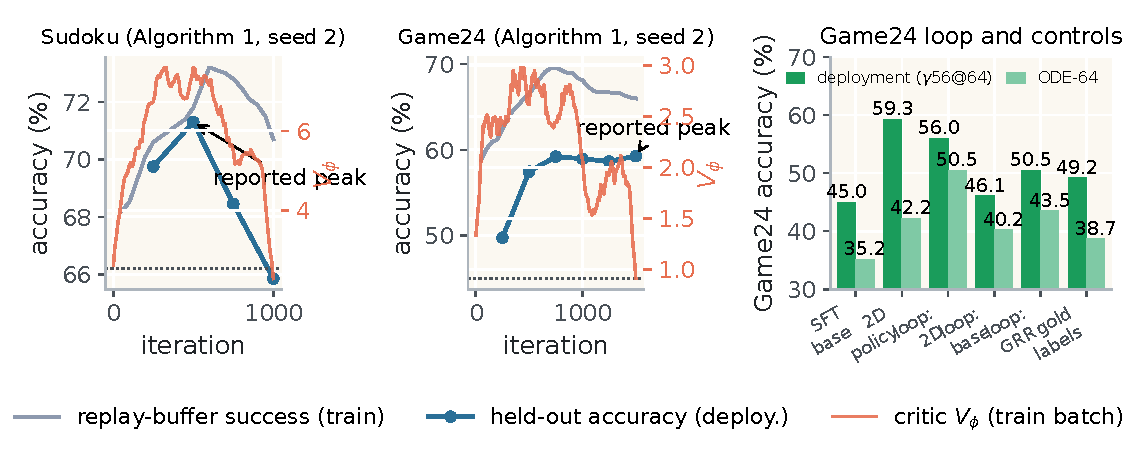
\includegraphics[width=0.66\linewidth]{figures/fig_dynamics_loop.pdf}
\caption{Left, middle: replay-buffer success (grey), critic value (red) and held-out accuracy (blue) for two \jpc{} runs; every run eventually enters a regime where the critic's value drifts while held-out accuracy falls, and the recipe keeps the held-out peak. Right: the loop on Game24 at the deployment and ODE-64 samplers (base, 2D-critic policy, loop from that policy, loop from the base).}
\label{fig:curves}
\end{figure}
